\chapter{High-Level Overview}
\label{cha:high-level-overview}
\begin{quote}
By a small sample we may judge the whole piece. --- Miguel de Cervantes Saavedra
\end{quote}
\section{Interacting with PyPedal}
\label{sec:interacting}
\index{interacting with PyPedal}
There are two ways to interact with \PyPedal{}: interactively\index{interacting with PyPedal!interactively} from a Python command line, and programmatically\index{interacting with PyPedal!programmatically} using a script that is run using the Python interpreter.  The latter is preferred to the former for any but trivial examples, although it is useful to work with the command line while learning how to use \PyPedal{}.  A number of sample programs are included with the \PyPedal{} distribution. %Examples of both styles of interaction may be found in the tutorial (Chapter \ref{cha:tutorial}).
\section{The PyPedal Object Model}
\label{sec:pypedal-objects}
\index{objects}
At the heart of \PyPedal{} are four different types of objects.  These objects
combine data and the code that operate on those data into convenient packages.
Although most \PyPedal{} users will only work directly with one or two of these
objects it is worthwhile to know a little about each of them.  An instance of the
\class{NewPedigree} class stores a pedigree read from an input file, as well as
metadata about that pedigree.  The pedigree is a Python list of \class{NewAnimal}
objects.  Information about the pedigree, such as the number and identity of founders,
is contained in an instance of the \class{PedigreeMetadata} class.

The fourth \PyPedal{} class, \class{New{AM}atrix}, is used to manipulate numerator
relationship matrices (NRM).  When working with large pedigrees it can take a long
time to compute the elements of a NRM, and having an easy way to save and restore
them is quite convenient.

\PyPedal{} also provides \class{LightAnimal} and \class{SimAnimal} objects. \class{LightAnimal}s
are intended for use with the graph theoretic routines provided in \module{pyp_network} and lack
many of the attributes of \class{NewAnimal} objects, such as names, breeds, and alleleotypes.
\class{SimAnimal}s are intended for internal use only by the pedigree simulation routines.

A detailed explanation of each class is provided in Chapter \ref{cha:using-pypedal-objects}.
\section{Program Structure}
\label{sec:overview-program-structure}
\index{program structure}
\PyPedal{} programs load pedigrees from files and operate on those pedigrees.  A program consists of four basic parts: a header, an options section, pedigree creation, and pedigree operations.  The program header is used to import modules used in that program, and may include any Python module available on your system.  You must import a module before you can use it:
\begin{verbatim}
# Program header -- load modules used by a program
from PyPedal import pyp_newclasses
from PyPedal import  pyp_metrics
\end{verbatim}
You should only import modules that you are going to use in your program; you do not need to import every \PyPedal{} module in every program you write.

\PyPedal{} recognizes a number of diffferent options that are used to control its behavior (Section \ref{sec:pypedal-options}).  Before you can load your pedigree into a \PyPedal{} object you must provide a pedigree file name (\samp{pedname}) and a pedigree format string (\samp{pedformat}).  This is done by either creating a Python dictionary and passing it as a parameter when \method{pyp_newclasses.loadPedigree()} is called or by specifying a configuration file\index{configuration file} name.  For example, here is how you would create and populate an options dictionary:
\begin{verbatim}
options = {}
options['messages'] = 'verbose'
options['renumber'] = 0
options['pedfile'] = 'new_lacy.ped'
options['pedformat'] = 'asd'
options['pedname'] = 'Lacy (1989) Pedigree'
\end{verbatim}
The syntax used in a configuration file is similar.  Consider the file \file{options.ini}, which contains the same options as set in the \var{options} dictionary in the previous example:
\begin{verbatim}
# options.ini
# This is an example of a PyPedal configuration file
messages = verbose
renumber = 0
pedfile = new_lacy.ped
pedformat = asd
pedname = Lacy (1989) Pedigree
\end{verbatim}
More details on configuration files are provided in Section \ref{sec:pypedal-options-file}.

You may name your dictionary or configuration file whatever you like; the examples in this manual, as well as those distributed with \PyPedal{}, use the name \samp{options}.  Once you have defined your options to is time to load your pedigree.  This is as simple as calling \function{pyp_newclasses.NewPedigree()}:
\begin{verbatim}
example = pyp_newclasses.loadPedigree(options)
\end{verbatim}
If you would like to use a configuration file to set your pedigree options, supply the configuration file name using the \var{optionsfile} keyword:
\begin{verbatim}
example = pyp_newclasses.loadPedigree(optionsfile='options.ini')
\end{verbatim}
Once you have loaded your pedigree file into a \class{NewPedigree} object you can unleash the awesome power of a fully-functional \PyPedal{} installation on it.  For example, calculating the effective number of founders in your pedigree using Lacy's \citeyear{ref640} exact method is as simple as:
\begin{verbatim}
pyp_metrics.effective_founders_lacy(example)
\end{verbatim}
Example programs that demonstrate how to use many of the features of \PyPedal{} are included in the \samp{examples} directory of the distribution.
\section{Options}
\label{sec:pypedal-options}
\index{options}
Many aspects of \PyPedal{}'s operation can be controlled using a series of options.  A complete list of these options, their defaults, and a brief desription of their purpose is presented in Table \ref{tbl:options}.  Options are stored in a Python dictionary that you must create in your programs.  You must specify values for the \var{pedfile} and \var{pedformat} options; all others are optional.  \var{pedfile} is a string containing the name of the file from which your pedigree will be read.  \var{pedformat} is a string containing a pedigree format code (see section \ref{sec:pedigree-format-codes}) for each column in the datafile in the order in which those columns occur.  The following code fragement demonstrates how options are specified.
\begin{verbatim}
options = {}
options['messages'] = 'verbose'
options['renumber'] = 0
options['counter'] = 5
options['pedfile'] = 'new_lacy.ped'
options['pedformat'] = 'asd'
options['pedname'] = 'Lacy Pedigree'
example = pyp_newclasses.loadPedigree(options)
\end{verbatim}
First, a dictionary named \var{options} is created; you may use any name you like as long as it is a valid Python variable name.  Next, values are assigned to several options.  Finally, \var{options} is passed to \function{pyp\_newclasses.loadPedigree()}, which requires that you pass it either a dictionary of options or a configuration file name.  If you do not provide one of these, \PyPedal{} will halt with an error.

A single \PyPedal{} program may be used to read one or more pedigrees.  Each pedigree that you read must be passed its own dictionary of options.  The easiest way to do this is by creating a dictionary with global options.  You can then customize the dictionary for each pedigree you want to read.  Once you have created a \PyPedal{} pedigree by calling \function{pyp\_newclasses.NewPedigree(options)} you can change the options dictionary without affecting that pedigree because it has a separate copy of those options stored in its \member{kw} attribute.  The following code fragment demonstrates how to read two pedigree files using the same dictionary of options.
\begin{verbatim}
options = {}
options['messages'] = 'verbose'
options['renumber'] = 0
options['counter'] = 5

if __name__ == '__main__':
#   Read the first pedigree
    options['pedfile'] = 'new_lacy.ped'
    options['pedformat'] = 'asd'
    options['pedname'] = 'Lacy Pedigree'
    example1 = pyp_newclasses.loadPedigree(options)
#   Read the second pedigree
    options['pedfile'] = 'new_boichard.ped'
    options['pedformat'] = 'asdg'
    options['pedname'] = 'Boichard Pedigree'
    example2 = pyp_newclasses.loadPedigree(options)
\end{verbatim}
Note that \var{pedformat} only needs to be changed if the two pedigrees have different formats.  Only \var{pedfile} \emph{has} to be changed at all.

All pedigree options other than \var{pedfile} and \var{pedformat} have default values.  If you provide a value that is invalid the option will revert to the default.  In most cases, a message to that effect will also be placed in the log file.
\begin{center}
    \tablecaption{Options for controlling PyPedal.}
    \tablefirsthead{\hline Option & Default & Note(s) \\ \hline}
    \tablehead{\hline Option & Default & Note(s) \\ \hline}
    \tabletail{\hline \multicolumn{3}{l}{\small\sl continued on next page} \\ \hline}
    \tablelasttail{\hline}
    \label{tbl:options}
    \index{options!list}
    \begin{xtabular}{l|l|p{4in}}
	alleles\_sepchar  & '/'          & The character separating the two alleles in an animal's allelotype. \var{alleles\_sepchar} CANNOT be the same as \var{sepchar}! \\
	animal\_type  & 'new'            & Indicates which animal class should be used to instantiate animal records, \class{NewAnimal} or \class{LightAnimal} (`new'|`light'). \\
	counter          & 1000          & How often should \PyPedal{} write a note to the screen when reading large pedigree files. \\
	database\_debug  & False         & Toggle debugging messages in the database module on and off. \\
	database\_host   & 'localhost'   & The server on which the database is running. \\
	database\_name   & 'pypedal'     & The name of the database to be used. \\
	database\_passwd & 'anonymous'   & The password needed to connect to your database. \\
	database\_port   & ''            & The port on which your databse is listening for connections (needed only for Postgres). \\
	database\_table  & 'filetag'     & The name of the database table to which the current pedigree will be written. \\
	database\_type   & 'sqlite'      & The type of database you are using ('mysql'|'postgres'|'sqlite'). \\
	database\_user   & 'anonymous'   & The name of a user with access rights to your database.  \\
	default\_fontsize & 10           & Specifies the default font size used in \module{pyp   \_graphics}. If the font size cannot be cast to an integer, it is set to the default value of 10. Font sizes less than 1 are set to the default of 10. \\
	default\_report   & filetag      & Default report name for use by \module{pyp\_reports}. \\
	default\_unit     & 'inch'       & The default unit of measurement for report generation ('cm'|'inch'). \\
	debug\_messages  & 0            & Indicates whether or not \PyPedal{} should print debugging information. \\
	f\_computed       & 0            & Indicates whether or not coefficients of inbreeding  have been computed for animals in the current pedigree.  If the pedigree format string includes \character{f} this will be set to 1; it is also set to 1 on a successful return from \function{pyp\_nrm/inbreeding()}. \\
	file\_io         & 1            & When true, routines that can write results to output files will do so and put messages in the program log to that effect. \\
	filetag          & pedfile      & \var{filetag} is a descriptive label attached to output files created when processing a pedigree.  By default the filetag is based on \var{pedfile}, minus its file extension. \\
	form\_nrm        & 0            & Indicates whether or not to form a NRM and bind it to the pedigree as an instance of a \class{NewAMatrix} object. \\
	foundercoi	 & 0		& Tells \function{pyp\_nrm.fast\_a\_matrix()} whether or not to use coefficients of inbreeding from the pedigree to augment the diagonals for founders.\\
	gen\_coeff       & 0            & When nonzero, calculate generation coefficients using the method of Pattie \citeyear{Pattie1965} and store them in the \member{gen\_coeff} attribute of a \class{NewAnimal} object.  The inferred generation stored in the \member{igen} attribute will be the \member{gen\_coeff} rounded to the nearest 0.5.  When zero, the \member{gen\_coeff} is -999. \\
	has\_header	 & 0		& When 1, the first row of the pedigree file is converted to a comment because it is a list of column names rather than data. If you are using a configuration file, you \emph{must} enclose the comma in double quotation marks (e.g., \code{has_header = ``,''}). \\
	log\_long\_filenames & 0        & When nonzero, long logfile names will be used, which means that log file names will include datestamps. \\
	log\_ped\_lines  & 0            & When $>$ 0 indicates how many lines read from the pedigree file should be printed in the log file for debugging purposes. \\
	logfile          & filetag.log  & The name of the file to which \PyPedal{} should write messages about its progress. \\
	matrix\_type	 & 'dense'	& Select between dense and sparse matrices.\\
	messages         & 'verbose'    & How chatty \PyPedal{} should be with respect to messages to the user.  'verbose' indicates that all status messages will be written to STDOUT, while 'quiet' suppresses all output to STDOUT. \\
	missing\_bdate    & '01011900'   & Default birth date. \\
	missing\_breed    & 'Unknown\_Breed'    & Default breed name.\\
	missing\_byear    & 1900         & Default birth year.\\
	missing\_herd	 & 'Unknown\_Herd'	& Default herd identifier.\\
	missing\_name     & 'Unknown\_Name'    & Default animal name.\\
	missing\_parent  & 0            & Indicates what code is used to identify missing/unknown parents in the pedigree file. \\
	missing\_sex	 & 'u'		& Default sex code.\\
	newanimal\_caller  & 'loader'   & Internal parameter needed for addanimal() to work correctly with ASD pedigrees. \\
	nrm\_format      & 'text'       & Format to use when writing an NRM to a file ('text'|'binary'). Array elements in text files are separated by \var{sepchar}.\\
	nrm\_method      & 'nrm'        & Specifies that an NRM formed from the current pedigree as an instance of a \class{NewAMatrix} object should ('frm') or should not ('nrm') be corrected for parental inbreeding. \\
	paper\_size       & 'letter'     & Default paper size for printed reports ('A4'|'letter'). \\
	pedcomp          & 0            & When 1, calculate pedigree completeness using pedcomp\_gens generations of pedigree. \\
	pedcomp\_gens    & 3            & Number of generations of pedigree to use when calculating pedigree completeness. \\
	pedfile          & None         & File from which pedigree is read; must provided unless you are simulating a pedigree. Defaults to 'simulated_pedigree' for simulated pedigrees. \\
	pedformat        & 'asd'        & See \ref{sec:pedigree-format-codes} for details. \\
	pedname          & 'Untitled'   & A name/title for your pedigree. \\
	pedgree\_is\_renumbered & 0     & Indicates whether or not the pedigree has been renumbered. \\
	pedigree\_summary & 1           & Indicates whether or not the pedigree loading details and summary are printed to STDOUT.  Output is only written if \var{message} is set to `verbose'. \\
	renumber         & 1            & Renumber the pedigree after reading from file (0/1). \\
	reorder 	 & 0		& Reorder the pedigree after reading from file (0/1). \\
	reorder\_max\_rounds & 100	& Maximum number of passes to use when reordering the pedigree. \\
	sepchar          & ' '          & The character separating columns of input in the pedfile. \\
	set\_ancestors   & 0            & Iterate over the pedigree to assign ancestors lists to parents in the pedigree (0/1). \\
	set\_alleles     & 0            & Assign alleles for use in gene-drop simulations (0/1). \\
	set\_generations & 0            & Iterate over the pedigree to infer generations (0/1). \\
	set\_offspring   & 0            & Assigns offspring to their parent(s)'s unknown sex offspring list. \\
	set\_sexes       & 0            & Iterate over the pedigree to assign sexes to all animals in the pedigree (0/1). \\
	simulate\_fs     & 0            & Flag indicating whether or not full-sib matings are allowed. \\
	simulate\_g      & 3            & Number of distinct generations in the simulated pedigree. \\
	simulate\_ir     & 0.0          & Immigration rate, the rate at which new founders with unknown parents enter the population. \\
	simulate\_mp     & 0            & Flag indicating whether or not simulated animals may have missing parents. \\
	simulate\_n      & 15           & Total number of animals in simulated pedigree, including founders. \\
	simulate\_nd     & 4            & Number of initial founder dams in pedigree. \\
	simulate\_ns     & 4            & Number of initial founder sires in pedigree. \\
	simulate\_pedigree & 0          & Option to simulate a pedigree rather that load one from a file. All other simulation-related variables are ignored when this is not set to 1. \\
	simulate\_pmd    & 100          & Maximum number of draws allowed when trying to sample parents that comply with all restrictions. \\
	simulate\_po     & 0            & Flag indicating whether or not parent-offspring matings are allowed. \\
	simulate\_save   & 0            & Flag indicating whether or not the simulated pedigree should be written to a file after it is created. \\
	simulate\_sr     & 0.5          & Sex ratio in simulated pedigree; < 0.5 gives more females, > 0.5 gives more males. \\
	slow\_reorder    & 1            & Option to override the slow, but more correct, reordering routine used by PyPedal by default (0/1).  ONLY CHANGE THIS IF YOU REALLY UNDERSTAND WHAT IT DOES!  Careless use of this option can lead to erroneous results. \\
    \end{xtabular}
\end{center}
\subsection{Configuration Files}
\label{sec:pypedal-options-file}
\index{configuration files}
The Dict4Ini\index{Dict4Ini} module (\url{http://cheeseshop.python.org/pypi/Dict4Ini/0.4}) is used to process configuration files, and in included with the distribution so that you do not need to download and install it.  Dict4Ini objects can be addressed as though they are standard Python dictionaries, which made it very easy to add configuration file support to \PyPedal{}.  Configuration files consist of simple \emph{keyword = value} pairs on separate lines\footnote{Please note that the Dict4Ini documentation referrs to sections.  Sections are very commonly used in configuration files, but \PyPedal{} does not use them.}, and may include comments.
\begin{verbatim}
# new_options.ini
# This is an example of a PyPedal configuration file.
pedfile = new_lacy.ped
pedformat = asd
pedname = Lacy Pedigree
\end{verbatim}
If neither an options dictionary nor a configuration file name is provided, \function{pyp_newclasses.loadPedigree()} will try and load the file named \file{pypedal.ini}.
\section{Pedigree Files}
\label{sec:pedigree-files}
\index{pedigree files}
Pedigree files consist of plain-text files (also known as ASCII or flatfiles) whose rows contain
records on individual animals and whose columns contain different variables.  The columns are
delimited (separated from one another) by some character such as a space or a tab (\textbackslash{}t).  Pedigree
files may also contain comments (notes) about the pedigree that are ignored by \PyPedal{}; comments
always begin with an octothorpe (\#).  For example, the following pedigree contains records for 13
animals, and each record contains three variables (animal ID, sire ID, and dam ID):
\begin{verbatim}
# This pedigree is taken from Boichard et al. (1997).
# Each records contains an animal ID, a sire ID, and
# a dam ID.
1 0 0
2 0 0
3 0 0
4 0 0
5 2 3
6 0 0
7 5 6
8 0 0
9 1 2
10 4 5
11 7 8
12 7 8
13 7 8
\end{verbatim}
When this pedigree is processed by \PyPedal{} the comments are ignored.  If you need to change the
default column delimiter \index{column delimiter}, which is a space (' '), set the \var{sepchar} option to the desired
value.  For example, if your columns are tab-delimited you would set the option as:
\begin{verbatim}
options['sepchar'] = '\t'
\end{verbatim}
Options are discussed at length in section \ref{sec:pypedal-options}. \PyPedal{} also provides tools for pedigree simulation, which are discussed in section \ref{sec:pedigree-simulation}. More details about pedigree input may be found in Chapter \ref{cha:inputoutput}.
\subsection{Pedigree Format Codes}
\label{sec:pedigree-format-codes}
\index{pedigree format codes}
Pedigree format codes consisting of a string of characters are used to describe
the contents of a pedigree file.  The simplest pedigree file that can be read by \PyPedal{}
is shown above; the pedigree format for this file is \var{asd}.  A pedigree format is required
for reading a pedigree; there is no default code used, and \PyPedal{} wil halt with an error if you
do not specify one.  You specify the format using an option statement at the start of your program:
\begin{verbatim}
options['pedformat'] = 'asd'
\end{verbatim}
Please note that the format codes are case-sensitive, which means that \character{a} is considered to be a different code than \character{A}.  The codes currently recognized by \PyPedal{} are listed in Table \ref{tbl:pedigree-format-codes}.

As noted, all pedigrees must contain columns corresponding to animals, sires, and dams, either in the 'asd' or 'ASD' formats (it is not recommended that you mix them such as in 'AsD').  Pedigree codes should be entered in the same order in which the columns occur in the pedigee file.  The character that separates alleles when the 'L' format code is used cannot be the same character used to separate columns in the pedigree file.  If you do use the same character, \PyPedal{} will write an error message to the log file and screen and halt.  The herd column type simply refers to a management group identifier, and can
correspond to a herd, flock, litter, etc.

If you used an earlier version of \PyPedal{} you may have added a pedigree format string, e.g. \texttt{"\% asd"}, to your pedigree file(s).  You no longer need to include that string in your pedigrees, and if \PyPedal{} sees one while reading a pedigree file it will ignore it.

Note that if your pedigree file uses strings for animal, sire, and dam IDs (the ASD pedigree format codes) you may need to override the \var{missing\_parent} option, which is \character{0} by default.  For example, the pedigree file shown in Figure \ref{fig:boichard-pedigree-basic} uses \var{animal0} to denote unknown parents.  If \samp{options['missing\_parent'] = 'animal0'} is not set before the pedigree file is loaded missing parents will be treated as animals with unknown parents, rather than as unknown parents.
\begin{center}
    \tablecaption{Pedigree format codes.}
    \tablefirsthead{\hline Code & Description \\ \hline}
    \tablehead{\hline Code & Description \\ \hline}
    \tabletail{\hline \multicolumn{2}{l}{\small\sl continued on next page} \\ \hline}
    \tablelasttail{\hline}
    \label{tbl:pedigree-format-codes}
    \index{pedigree format codes!list}
    \begin{xtabular}{l|p{4in}}
	a & animal ('a' or 'A' REQUIRED)\\
	s & sire ('s' or 'S' REQUIRED)\\
	d & dam ('d' or 'D' REQUIRED)\\
	y & birthyear (YYYY)\\
	e & age\\
	f & coefficient of inbreeding\\
	g & generation\\
	h & herd\\
	l & alive (1) or dead (0)\\
	n & name\\
	p & Pattie's \citeyear{Pattie1965} generation coefficient\\
	r & breed\\
	u & user-defined field (string)\\
	b & birthdate in "MMDDYYYY" format\\
	x & sex\\
	A & animal ID as a string (cannot contain \samp{sepchar})\\
	S & sire ID as a string (cannot contain \samp{sepchar})\\
	D & dam ID as a string (cannot contain \samp{sepchar})\\
	H & herd as a string (cannot contain \samp{sepchar})\\
	L & alleles (two alleles separated by a non-null character)\\
	Z & indicates a column that should be skipped (one allowed per pedigree)\\
    \end{xtabular}
\end{center}
\section{Renumbering a Pedigree}
\label{sec:renumbering}
\index{renumbering pedigrees}
Whenever you load a pedigree into \PyPedal{} a list of offspring is attached to the record for each animal in the pedigree file.  If you renumber the pedigree at the time it is loaded, there is no problem.  However, if you do not renumber a pedigree at load time and choose to renumber it later in your session you must be careful.  The API documentation may lead you to believe that
\begin{verbatim}
    example.pedigree = pyp_utils.renumber()
\end{verbatim}
is the correct way to renumber the pedigree, but that is not correct.  The pedigree should always be numbered as:
\begin{verbatim}
    example.kw['renumber'] = 1
    example.renumber()
\end{verbatim}
If you are seeing strange results when trying to cross-reference offspring to their parents check to make sure that you have not incorrectly renumbered your pedigree.
\subsection{Animal Identification}
\label{sec:renumbering-animal-id}
\index{renumbering pedigrees!animal identification}
A detailed explanation of animal identification cross-references is provided in Section \ref{sec:methodology-id-mapping}.
\section{Logging}
\label{sec:logging}
\index{logging}
\PyPedal{} uses the \module{logging} module that is part of the Python standard library to record events during pedigree processing.  Informative messages, as well as warnings and errors, are written to the logfile, which can be found in the directory from which you ran \PyPedal{}.  An example of a log from a successful (error-free) run of a program is presented below:
\begin{verbatim}
Fri, 06 May 2005 10:27:22 INFO     Logfile boichard2.log instantiated.
Fri, 06 May 2005 10:27:22 INFO     Preprocessing boichard2.ped
Fri, 06 May 2005 10:27:22 INFO     Opening pedigree file
Fri, 06 May 2005 10:27:22 INFO     Pedigree comment (line 1): # This pedigree is
                                   taken from Boicherd et al. (1997).
Fri, 06 May 2005 10:27:22 INFO     Pedigree comment (line 2): # It contains two
                                   unrelated families.
Fri, 06 May 2005 10:27:22 WARNING  Encountered deprecated pedigree format string
                                   (% asdg) on line 3 of the pedigree file.
Fri, 06 May 2005 10:27:22 WARNING  Reached end-of-line in boichard2.ped after reading
                                   23 lines.
Fri, 06 May 2005 10:27:22 INFO     Closing pedigree file
Fri, 06 May 2005 10:27:22 INFO     Assigning offspring
Fri, 06 May 2005 10:27:22 INFO     Creating pedigree metadata object
Fri, 06 May 2005 10:27:22 INFO     Forming A-matrix from pedigree
Fri, 06 May 2005 10:27:22 INFO     Formed A-matrix from pedigree
\end{verbatim}
The \texttt{WARNING}s let you know when something unexpected or unusual has happened, although you might argue that coming to the end of an input file is neither.  If you get unexpected results from your program make sure that you check the logfile for details -- some subroutines return default values such as -999 when a problem occurs but do not halt the program.  Note that comments found in the pedigree file are written to the log, as are deprecated pedigree format strings used by earlier versions of \PyPedal{}.  When an error from which \PyPedal{} cannot recover occurs a message is written to both the screen and the logfile.  We can see from the following log that the number of columns in the pedigree file did not match the number of columns in the pedigree format string.
\begin{verbatim}
Thu, 04 Aug 2005 15:36:18 INFO     Logfile hartlandclark.log instantiated.
Thu, 04 Aug 2005 15:36:18 INFO     Preprocessing hartlandclark.ped
Thu, 04 Aug 2005 15:36:18 INFO     Opening pedigree file
Thu, 04 Aug 2005 15:36:18 INFO     Pedigree comment (line 1): # Pedigree from van
                                   Noordwijck and Scharloo (1981) as presented
Thu, 04 Aug 2005 15:36:18 INFO     Pedigree comment (line 2): # in Hartl and Clark
                                   (1989), p. 242.
Thu, 04 Aug 2005 15:36:18 ERROR    The record on line 3 of file hartlandclark.ped
                                   does not have the same number of columns (4) as
                                   the pedigree format string (asd) says that it
                                   should (3). Please check your pedigree file and
                                   the pedigree format string for errors.
\end{verbatim}
There is no sensible ``best guess'' that \PyPedal{} can make about handling this situation, so it halts.  There are some cases where \PyPedal{} does ``guess'' how it should proceed in the face of ambiguity, which is why it is always a good idea to check for \texttt{WARNING}s in your logfiles.
\section{Simulating Pedigrees}
\label{sec:pedigree-simulation}
\index{pedigree simulation}
\PyPedal{} is capable of simulating pedigrees using am algorithm based on the \method{Pedigree::sample} method in Matvec 1.1a (\url{http://statistics.unl.edu/faculty/steve/software/matvec/}), although the implementation in \class{NewPedigree} is all original code. A pedigree is simulated when the \member{simulate\_pedigree} flag is set, and is the only case in which a \member{pedfile} does not need to be provided to \PyPedal{}. All simulated pedigrees have the code `asdxg' and are \emph{not} renumbered. The options used to control pedigree simulation are presented in Table \ref{tbl:options}.

The basic structure of a simulated pedigree is determined by the total number of simulated animals (\member{simulate\_n}), founder sires (\member{simulate\_ns}) and dams (\member{simulate\_nd}), and the number of distinct generations in the pedigree (\member{simulate\_g}). Populations can be closed or open based on the value of \member{simulate\_ir}; when the immigration rate is $>$ 0 that proportion of new animals will be immigrants with unknown parents. The sex ratio can be altered by changing \member{simulate\_sr}; values $<$ 0.5 will result in more females than males, and values $>$ 0.5 will result in more males than females. By default, \method{NewPedigree.simulate} produces a three-generation pedigree with 15 animals descended from 4 founder sires and 4 founder dams (Figure \ref{fig:example-simulated-pedigree}).
\begin{figure}
  \begin{center}
    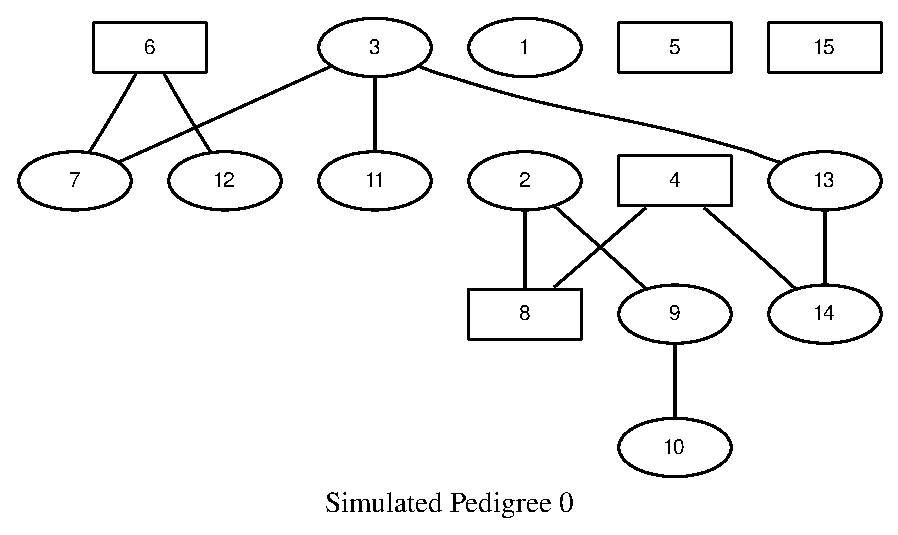
\includegraphics[width=4in]{simulatedPedigree.eps}
    \caption{Simulated pedigree using default options}
    \label{fig:example-simulated-pedigree}
  \end{center}
\end{figure}
\var{simulate\_mp} is a flag indicating whether or not simulated animals may have missing parents. When missing parents are allowed, animals may have no, one, or both parents unknown. The related parameter, \var{simulate\_pmd}, specifies the number of times parents should be sampled at random when trying to satisfy all of the simulation constraints. If parents are sampled \var{simulate\_pmd} times without satisfying the rules in place, both parents are set to missing, even if missing parents are not permitted. Other constraints include allowing/forbidding parent-offspring (\var{simulate\_po}) and/or full sib (\var{simulate\_fs}) matings.
